\documentclass[twocolumn]{aastex61}
\usepackage{bm}
\usepackage{amsmath}
\usepackage{color}

\newcommand\teff{T_{\rm eff}}
\newcommand\logg{\log{g}}
\newcommand\feh{[\rm{Fe}/\rm{H}]}
\newcommand\mh{[\rm{M}/\rm{H}]}
\newcommand{\luminosity}{L_\circ}
\newcommand{\radius}{R_\circ}


\newcommand{\project}[1]{\textsl{#1}}
\newcommand{\package}[1]{\texttt{#1}}
\newcommand{\acronym}[1]{{\small{#1}}}
\newcommand{\Gaia}{\project{Gaia}}
\newcommand{\gaia}{\project{gaia}}
\newcommand{\todo}[1]{\textcolor{red}{#1}}
\newcommand{\rp}{\textsl{rp}}
\newcommand{\bp}{\textsl{bp}}


\newcommand{\NumberOfStellarMultiples}{XXX}
\newcommand{\NumberOfStellarSingles}{XXX}


\newcommand{\GaiaRVE}{\sigma_{\mathrm{V}_\mathrm{R}}^\mathrm{MTA}}
\newcommand{\RVJitter}{\sigma(\mathrm{V}_\mathrm{R}^{t})}

\received{2018 XX XX}
\revised{2018 XX XX}
\accepted{2018 XX XX}


\submitjournal{AAS Journals}

\shorttitle{Stellar multiplicity}
\shortauthors{Casey et al.}

\begin{document}

\title{Detection and partial characterisation of stellar multiplicity with Gaia}

\correspondingauthor{Andrew R. Casey}
\email{andrew.casey@monash.edu}

% Some order of the following authors (order is TBD)

\author[0000-0003-0174-0564]{Andrew R. Casey}
\affiliation{School of Physics \& Astronomy, 
			 Monash University,
			 Wellington Rd, Clayton 3800, Victoria, Australia}
\affiliation{Faculty of Information Technology, 
			 Monash University, 
			 Wellington Rd, Clayton 3800, Victoria, Australia}

\author[0000-0002-9328-5652]{Daniel Foreman-Mackey}
\affiliation{Flatiron Institute, 
			 162 Fifth Ave, New York, NY 10010, USA}

\author[0000-0003-2866-9403]{David W. Hogg}
\affiliation{Center for Cosmology and Particle Physics, Department of Physics,
    		 New York University, 
		  	 726 Broadway, New York, NY 10003, USA}
\affiliation{Center for Data Science, 
			 New York University, 60 Fifth Ave, New York, NY 10011, USA}
\affiliation{Max-Planck-Institut f\"ur Astronomie, 
			 K\"onigstuhl 17, D-69117 Heidelberg}
\affiliation{Flatiron Institute,
			 162 Fifth Ave, New York, NY 10010, USA}

\author[0000-0003-3494-343X]{Carles Badenes}
\affiliation{Department of Physics and Astronomy, 
			 University of Pittsburgh, 
			 3941 O'Hara Street, Pittsburgh, PA 15260, USA}

\author[0000-0003-0872-7098]{Adrian M. Price-Whelan}
\affiliation{Department of Astrophysical Sciences, 
			 Princeton University, 
			 Princeton, NJ 08544, USA}


\begin{abstract}
The properties and occurrence rate of stellar multiples (e.g., binaries, triples) 
underpins much of astrophysics. Precisely measuring these quantities is challenging
and observationally demanding. Here we use \Gaia\ data to detect and partially 
characterise \NumberOfStellarMultiples\ stellar multiple systems based on excess 
astrometric jitter, excess radial velocity jitter, the absence of reported radial
velocities, photometry, and intrinsic luminosity.
\todo{We show that astrometric and radial velocity jitter can be calibrated to
estimate inclination angles (and directly constrain companion masses) for thousands 
of systems.}
Comparisons with literature surveys on stellar multiplicity demonstrate that we 
reliably detect binary systems with orbital periods up to $\approx$3.5\,yr. 
\todo{A comment on stellar multiplicity with stellar metallicity.}
\todo{A comment on stellar multiplicity in the field relative to clusters.}
\todo{A comment on systems with stellar remnants (e.g., NS/BHs).}
\end{abstract}


\keywords{(stars:) binaries: general, (stars:) binaries: spectroscopic, (stars:) binaries (including multiple): close, astrometry, techniques: radial velocities, methods: statistical}

\section{Introduction} \label{sec:intro}

Higher order stellar systems describes any stars that have at least one stellar 
companion (e.g., binaries, trinaries). The presence of stellar companions
introduces a number of complications to the inference of stellar and galactic
properties, but these factors are often ignored.

The \Gaia\ space telescope provides exquisite astrometry, photometry, and radial
velocity measurements over many years for million of point stars in our galaxy.
%These data provides an excellent opportunity to self-calibrate the errors in those
%measurements. 
When a point source has an unresolved stellar companion within some range of orbital
and stellar parameters, it is expected that there will be an anomalous excess in 
these measured properties relative to a single star of a similar type. This is
nothing new: astronomers have used radial velocity \citep{Butler:1996} and 
astrometric variations \citep{Muterspaugh:2010} and photometry \citep{someone} to infer the 
presence of stellar and exoplanet companions forever. However, the opportunity
presented by \Gaia\ is to infer the presence of stellar companions for millions
of point sources, across both hemispheres. No ground- or space-based instrument
has ever provided such an opportunity.

In this work we make use of photometry and astrometry (including radial motion)
measurements in the second \Gaia\ data release to infer the presence of stellar
companions for millions of point sources, and provide some basic characterisations
of these systems. In Section \ref{sec:method} we describe our methods, and in
Section \ref{sec:results} we outline our results in context of other stellar
multiplicity surveys. We include comparisons of binary properties between
clusters and the field, as a function of stellar properties (e.g., stellar
metallicity), and highlight some particularly noteworthy systems that would
benefit from immediate follow-up spectroscopic observations. 


\section{Method} \label{sec:method}

There are many ways that binaries can be reliably identified using \Gaia\
data, including radial velocity measurements, photometry, and astrometry.
These detection methods are sensitive to binary systems with different 
properties. Here we describe the absence of reported radial velocity in
\Gaia\ data can be used to deduce stellar multiples, before we describe
our model that incorporates measurements of radial velocity, astrometry, 
and photometry, to detect and characterise stellar multiples.

\subsection{SB2 Systems: Double-lined spectroscopic binaries}
\label{sec:sb2_methods}

Many sources in the second \Gaia\ data release do not have a reported radial 
velocity, despite being bright enough ($G \lesssim 13$) and in a suitable 
temperature range (e.g., between $\approx4000\,\textrm{K}$ and $\approx6500\,\textrm{K}$) 
for radial velocities to be measured \citep{Cropper:2018}. The principle reason 
why radial velocity measurements are \emph{not} reported for these stars is 
because the \Gaia/DPAC team have identified the source to be a double-lined 
spectroscopic binary (a so-called SB2-type system), either through a 
composition of two stellar sources present in the spectra, or from multiple 
(significant) modes in the cross-correlation function. In these situations it
is not sensible to report a point estimate of the radial velocity of the point 
source. For fainter or bluer sources, however, the radial velocity 
may not be reported simply because it is too faint, blue, or red. 


We calculated the completeness of radial velocity measurements (e.g., the
fraction of sources with reported radial velocities) as a function of all 
available source properties that might affect whether the radial velocity may
be reported or not. This included position ($\alpha$, $\delta$, $l$, $b$),
parallax, proper motions, apparent magnitudes, \bp\ - \rp\ colour, 
properties of the radial velocity templates, stellar parameters ($\teff$, $\radius$, $\luminosity$),
and other properties. The full list of properties investigated is described in
Appendix \ref{appendix:sb2}, with corresponding figures. 

In Figure \ref{fig:radial_velocity_completeness} we show the completeness as 
a function of some pertinent properties, which demonstrate that the radial 
velocity completeness is relatively flat until a source becomes too faint 
(low \rp\ flux), or is either too blue or too red. We adopt conservative 
limits for when the radial velocity completeness starts to drop with these 
properties, and we assume that any source within the following range of 
source parameters
\begin{eqnarray}
    \mathrm{phot\,\,rp\,\,mean\,\,flux} & \in & [10^{4}, 10^8] \nonumber \\
    \mathrm{bp-rp} & \in & [X, Y] 
    \label{eq:sb2_criteria}
\end{eqnarray}
\noindent{}is likely to be a double-lined spectroscopic binary (SB2) if no 
radial velocity is reported. That is to say that we are explicitly assuming
that if a point source meets the criteria in Equation \ref{eq:sb2_criteria} 
and does not have a reported radial velocity measurement, then the point 
source is an unresolved double-lined spectroscopic binary. In principle we 
could make more realistic attempts to model the radial velocity completeness as
a function of stellar properties rather than simply stating ``sources within
this parameter range should have radial velocities unless they are SB2 systems'',
but the radial velocity completeness within our specified range is reasonably
flat.


\todo{Some confirmation of this? The properties of SB2 candidate systems relative to others. Figure \ref{fig:sb2_histograms}.}


We stress that our sample of SB2 type systems is calculated (or rather, deduced)
separately to our calculations of multiplicity probability given the 
\emph{measured} quantities from \Gaia\ like radial velocity, astrometry, and
photometry. In Section \ref{sec:discussion} we detail some of the immediate
limitations or interpretations of this assumption, and we emphasise that the 
main conclusions of this work do not depend on SB2 systems. Nevertheless, we 
\emph{strongly} 
caution that our deductive inference of SB2 systems will be far more uncertain 
than the binary probabilities we derive from other information. Our indicator 
whether a star is likely a SB2 system likely suffers from more contamination
and lower completeness compared to the probabilities we derive from other information
(e.g., the radial velocity jitter, astrometric excess noise, and photometric 
colours), and the contamination and completeness likely vary over some
complex (unknown) function of parameter space. 




\begin{figure*}
	\includegraphics[width=1.0\textwidth]{../figures/sb2_rvs_completeness.pdf}
    \caption{Fraction of \Gaia\ sources with reported radial velocities
		     as a function of source properties. Within the adopted source
		     parameter ranges (gray; see Section \ref{sec:sb2_methods})
		     the radial velocity completeness is approximately flat.
		     We flag sources within this range that do not have reported 
		     radial velocities to be candidate SB2 systems.}
    \label{fig:sb2_rvs_completeness}
\end{figure*}




\begin{figure}
	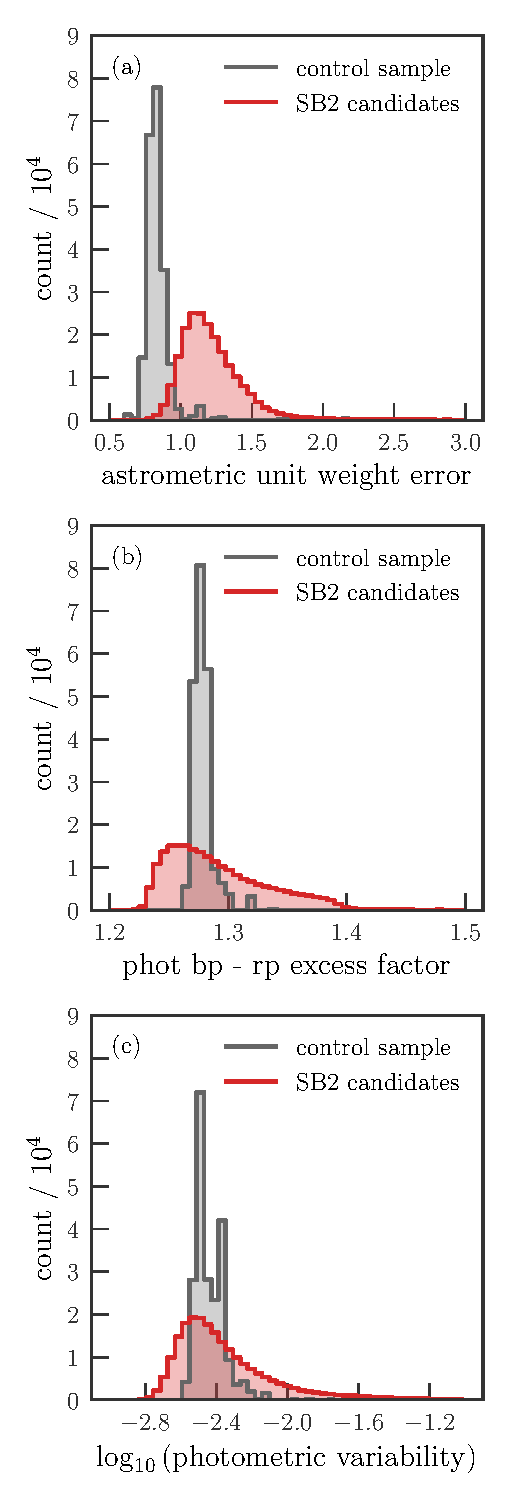
\includegraphics[width=0.4\textwidth]{../figures/sb2_histograms.pdf}
    \caption{Distribution of 
    			(a) astrometric unit weight error (see Eq. \ref{eq:astrometric_unit_weight_error}),
			%$u = \left(\chi_{al}^2/(N_{al} - 5)\right)^{1/2}$
			%		where $\chi_{al}^2$ and $N_{al}$ is the astrometric goodness-of-fit and number 
			%		of observations in the along-scan direction, respectively (columns 
			%			\texttt{astrometric\_chi2\_al} and \texttt{astrometric\_n\_obs\_al}), 
				(b) photometric \bp\ - \rp\ excess factor, 				
	 				and 
				(c) photometric \rp\ variability (see Eq. \ref{eq:photometric_variability})
			of candidate SB2 type systems relative to a control sample of the same size.}
    \label{fig:sb2_histograms}
\end{figure}



\begin{figure*}
	\includegraphics[width=1.0\textwidth]{../figures/sb2_sky_structure.pdf}
    \caption{Fraction of sources (per sky bin) without reported radial velocities
    		 for all sources with $G \lesssim 13$ (top) and sources in the ranges
		 	 specified by Eqs \ref{eq:sb2_ranges} (bottom), where we assert that a missing
			 radial velocity measurement signifies a likely SB2 candidate . The color scale is 
			 arbitrarily set to highlight structure, where black indicates a higher
			 fraction of sources do not have reported radial velocities. Crowding
			 in the galactic plane likely results in some sources not having radial
			 velocities reported. The large scale structure visible in both axes is
			 a combined effect of the initial \Gaia\ source list, the scanning law,
			 and star forming regions (i.e., where emission in the \ion{Ca}{2} 
			 triplet likely causes issues for radial velocity determination).}
    \label{fig:sb2_sky_structure}
\end{figure*}


% Figure: cross-match against a catalog of SB2 systems,... do we find all of
% 		  what they find from SB2 deductive inference alone? or do we miss
% 		  some SB2s in some parameter range?


\subsection{SB1 Systems: Single-lined spectroscopic binaries}
\label{sec:sb1_methods}

Radial velocity measurements are not available for individual epochs in the 
second \Gaia\ data release \citep{Lindegren:2018,Cropper:2018}, but a point estimate
and error in radial velocity is available for 7,224,631 sources \cite{Cropper:2018}.
% TODO: That's the value from the paper, but I think the true value is lower. Check.
The reported radial velocity error ($\GaiaRVE$; column name \texttt{radial\_velocity\_error}) 
is a function of the number of transits $N$ (i.e., the number of observations; 
represented by column \texttt{rv\_nb\_transits}) and the standard deviation among 
those $N$ measurements of radial velocity. This allows us to calculate the standard
deviation in radial velocity for each source, independent of the number of measurements,
which we will refer to as the \emph{radial velocity jitter} $\RVJitter$,
\begin{eqnarray}
\RVJitter = \sqrt{\frac{2N}{\pi}}\GaiaRVE \quad .
\end{eqnarray}



For a single star (without a significant mass companion) the source radial velocity
jitter represents the minimum uncertainty with which \Gaia\ can measure 
radial velocity for a star of that colour, apparent brightness, and absolute brightness.
However for stars with stellar companions and no evidence of double lines or binarity in the
cross-correlation-function, so-called SB1 type systems \citep{someone}, the
radial velocity jitter is a function of the orbital parameters and observation
epochs. We assume that the distribution of radial velocity jitter in the second
\Gaia\ data release is a mixture of two populations:

\begin{enumerate}
\item \emph{single-star systems}, where the radial velocity jitter represents the
      minimum radial velocity noise that \Gaia\ can measure for a star of that
      \bp\ - \rp\ colour, apparent \rp\ magnitude, and absolute \rp\ magnitude;
      
\item \emph{higher-order star systems}, where the radial velocity jitter is
      significantly above that for single-star systems of a similar colour, 
      apparent magnitude, and absolute magnitude.
\end{enumerate}

The mean radial velocity jitter of a single star will vary depending on the 
\bp\ - \rp\ colour of the source and the apparent magnitude. Similarly, the mean
radial velocity jitter of stellar \emph{multiples} will depend on the source 
colour and its position in the Hertzsprung-Russell diagram. For these reasons,
we must consider the radial velocity jitter of a source in context with other
sources that have a similar \bp\ - \rp\ colour, a similar apparent \rp\ magnitude,
and a similar absolute \rp\ magnitude. In principle if we knew the underlying
distribution and properties of stellar multiples then we could model how different
binary (and higher order) systems would be observable across the Hertszprung-Russell
diagram. 

We chose to adopt a non-parametric model for stellar multiplicity across the
Hertsprung-Russell diagram because we do not know the distribution of properties
of stellar multiples. Specifically, for each source we take the following steps:

\begin{enumerate}

	\item Select sources with similar \bp\ - \rp\ colours, a similar apparent \rp\
		  magnitude, and a similar absolute \rp\ magnitude.
		  		  
	\item We fit a two-component mixture model to the distribution of radial
		  velocity jitter for the subset of similar sources selected in Step 1.
		  
	\item Evaluate whether the source of interest is more consistent with being
		  drawn from the single star component (the normal distribution) or the
		  stellar multiple component (the log-normal distribution).
	
	\item For sources that are more consistent with being drawn from the stellar
		  multiple component, provide a partial characterisation of the system by
		  calculating the excess radial velocity jitter (above what is expected 
		  for a single star with similar observed properties), among other 
		  quantities.
		 
\end{enumerate}

We illustrate this procedure in Figure \ref{fig:npm_schematic}, where we demonstrate
how the distribution of source properties (e.g., radial velocity jitter) varies across
the Hertsprung-Russell diagram. While this model is flexible enough to describe varying
properties of single stars and stellar multiples, there are a number of explicit 
assumptions that go into this model:

\todo{assumptions}


\begin{figure*}
	
\includegraphics[width=1.0\textwidth]{../figures/todo.png}
    \caption{Illustration of the method we adopt for identifying and characterising
    		 stellar multiplicity across the Hertsprung-Russell diagram. For each
		 	 \Gaia\ source we select between 128 and 1024 sources that have
			 similar \bp\ - \rp\ colours, apparent \rp\ magnitudes, and absolute \rp\
			 magnitudes (Step 1). With these similar sources we fit a two-component
			 model to distinguish single star sources from stellar multiples (Step 2).
			 With the model parameters optimised from Step 2, we evaluate probability
			 of stellar multiplicity and partially characterise the higher order
			 systems by assuming binarity and estimating the system semi-amplitude (Step 3).}
    \label{fig:npm_schematic}
\end{figure*}

\subsubsection*{Step 1: Selecting similar sources}

We construct a $k$-dimensional tree \citep[k-d tree;][]{} for all sources in the
dimensions of \bp\ - \rp\ colour, apparent \rp\ magnitude, and absolute \rp\ magnitude.
When doing so we scale the dimensions such that 0.1\,mags in \bp\ - \rp\ colour is
approximately equal to 1 magnitude in apparent \rp\ magnitude and 1 magnitude in 
absolute \rp\ magnitude. We use this k-d tree for constructing the `ball' of similar
stars for every source.

We enforce a number of constraints when querying for similar stars. For each source
we require the `ball' in multi-dimensional space to include at least 128 sources.
We further require that the radius of the ball extends to at least 0.05\,mags in 
\bp\ - \rp\ colour, 0.5\,mags in apparent \rp\ magnitude, and 0.5\,mags in absolute
\rp\ magnitude. If the initial query of 128 points does not extend wide enough to
meet our constraints on minimum radius, we extend the radius (linearly in each scaled)
dimension until the minimum constraints on radii are met. Our minimum radii constraints
imply that there will be many (e.g., $>>128$) points returned in dense regions of the
Hertsprung-Russell diagram. In these situations we then subsample the selected points
to return a random 1024 sources in any ball, while enforcing our constraints on
minimum radii. As a result, the number of `similar' sources selected will range from
a minimum of 128 to a maximum of 1024, and the minimum radii constraints on various
dimensions are always maintained.


\subsubsection*{Step 2: Optimizing the two-component mixture}

We fit a two-component mixture model to the distribution of radial velocity jitter for
all similar sources selected through Step 1. This mixture model includes a normal
distribution to represent the intrinsic jitter for single stars, and a log-normal
distribution to represent stellar multiples. Specifically the model parameters include
a mixing weight parameter $\theta$ that is constrained between $(0, 1)$, the mean 
$\mu_{s}$ and standard deviation $\sigma_{s}$ of the normal distribution,
and the mean $\mu_{m}$ and standard deviation $\sigma_{m}$ of the 
log-normal distribution. For brevity we 

We assume a beta prior on $\theta$  such that $\theta \sim \mathcal{B}\left(5, 5\right)$
and we require $\sigma_{s}$ and $\sigma_{m}$ to be larger than zero.
Depending on the distribution of the radial velocity jitter, we often found this mixture
challenging to optimize because the log-normal distribution could easily account for 
most of the observed distribution, which tended the mixing weight to zero and implied
that all selected sources were stellar multiples. To avoid this situation we placed a
constraint on the mean of the log-normal distribution to ensure that the \emph{mode}
of the log-normal distribution is between $\mu_{s} + 1\sigma_{s}$ and
$\mu_{s} + 5\sigma_{s}$. The mode of the log-normal distribution is
$\exp\left(\mu_{m} - \sigma_{m}^2\right)$ such that
\begin{eqnarray}
	\mu_{s} + 5\sigma_{s} & > & \exp\left(\mu_{m} - \sigma_{m}^2\right) \label{eq:rvm_lower_bound} \\
	\mu_{s} + 1\sigma_{s} & < & \exp\left(\mu_{m} - \sigma_{m}^2\right) \label{eq:rvm_upper_bound} \quad .
\end{eqnarray}

However, we found that this constraint alone was insufficient. Often the mode would
be very close to the $\mu_{s} + 1\sigma_{s}$ lower bound, which implies that
the log-normal distribution is providing a considerable fraction of probability support
to sources with radial velocity jitter near the mean of the \emph{normal} distribution.
For this reason we chose to alter our lower bound constraint in that we also required
that at the mean of the normal distribution, the cumulative probability distribution
of the log-normal must be less than 10\% (let $q = 0.10$). The cumulative distribution 
function for the log-normal distribution is
\begin{eqnarray}
\textrm{CDF}(x|\mu_{m},\sigma_{m}) = \frac{1}{2} + \frac{1}{2}\textrm{erf}\left(\frac{\log{x} - \mu_{m}}{\sqrt{2}\sigma_{m}}\right) 
\end{eqnarray}

\noindent{}where \textrm{erf} is the standard error function. We use the approximation 
to the error function 
\begin{eqnarray}
	\textrm{erf}\left(x\right) \approx \tanh\left(\sqrt{\pi}\log{2}x\right)
\end{eqnarray}

\noindent{}and use the identity
\begin{eqnarray}
	\tanh^{-1}\left(x\right) = \frac{1}{2}\left[\log{\left(1 + x\right)} - \log{\left(1 - x\right)}\right]
\end{eqnarray}

\noindent{}to write our constraint on $\mu_{m}$ as
\begin{eqnarray}
	\mu_{m} & > & \log\mu_{s} + \frac{\sigma_{m}}{2\log{2}}\sqrt{\frac{2}{\pi}}\log{\left(\frac{1}{q} - 1\right)} \nonumber \\
	\mu_{m} & > & \log\mu_{s} + \frac{\sigma_{m}}{2\log{2}}\sqrt{\frac{2}{\pi}}\log{9} \label{eq:rvm_lower_bound2} \quad .
\end{eqnarray}

Incorporating the bounds from Equations \ref{eq:rvm_lower_bound}, \ref{eq:rvm_upper_bound},
and \ref{eq:rvm_lower_bound2} leads to the prior
\begin{eqnarray}
	\mu_{m} \sim \mathcal{U}\left(\alpha, \beta\right)
\end{eqnarray}

\noindent{}where:
\begin{eqnarray}
  \alpha & = & \max\left(\!
	\begin{aligned}
		\log{\left(\mu_{s} + 1\sigma_{s}\right)} + \sigma_{m}^2\\
		\log\mu_{s} + \frac{\sigma_{m}}{2\log{2}}\sqrt{\frac{2}{\pi}}\log{9}
	\end{aligned}\right) \\
  \beta & = & \log{\left(\mu_{s} + 5\sigma_{s}\right)} + \sigma_{m}^2 \quad .
\end{eqnarray}

We found these priors were sufficient to ensure numerical stability and efficiency.

Wherever possible we initialised the model parameters from nearby points (within the
ball selected by the k-d tree) where an optimised result already exists. This was primarily to minimise
computational cost; the initialisation did not have a noticeable impact on the
optimised result. We required the log probability and the gradient of the log
probability to reach machine precision before considering the optimisation
converged. After convergence, we queried to see if any points within the ball of
similar stars had not been optimized. If no result existed, we would next move to that
point. We refer to this process as \emph{swarm optimisation}, which we conducted in 
parallel, and illustrate in Figure \ref{fig:swarm_optimisation}.

\todo{To minimise computational cost we assigned the closest 8 stars with the result
from others}

\subsubsection*{Step 3: Evaluating probability and system properties}

 
\todo{Bayes factors for each dimension?}

\todo{source properties: semi-amplitude (easy)}

\todo{Can we recover period and eccentricity using The Joker?}




%For higher-order star systems with longer periods, we can still find that a
%stellar multiple system is more likely than a single star scenario, but our
%estimate of the orbital properties (e.g., the semi-amplitude $K$) will be biased
%to lower values because we have not fully sampled half of the orbital period.
%At even longer orbital periods, or for stellar multiples with mass ratios that
%produce a small velocity semi-amplitude $K$, under our assumptions these systems 
%may be classified as single-star systems because the intrinsic radial velocity variation is within the expected 
%variations for single stars of a similar apparent magnitude and colour. We 
%revisit this issue in Section \ref{sec:sb_limits}, where we explicitly define 
%the probability that a \Gaia\ source is a SB1-type system $p(\textrm{SB1}|y)$ 
%within defined limits of orbital period (and other orbital and source parameters). 
%Outside of this parameter range, we are insensitive to distinguishing single-star 
%systems from higher-order SB1-type systems.





\subsection{Unresolved near-equal mass binaries: photometry}
\label{sec:pb_methods}

If a binary system is observed nearly face-on (at an inclination angle 
$i \approx 0^\circ$) then there is will be no detectable excess radial 
velocity variations. In principle there may be detectable astrometric
variations, but most near-equal mass binaries would be detected more 
reliably through intrinsic magnitudes that are anomalously lower (brighter)
and bluer colours than what would be expected for a single star system.

\todo{How the fuck am I going to model this, exactly?}



\subsection{Astrometric binaries} \label{sec:method_astrometric_binaries}

Many higher-order star systems are unresolved point sources in \Gaia, but the
stellar companion(s) may have sufficient mass to measurably affect the tangential 
velocity of the primary and produce a detectable jitter in the astrometric 
positions. There are many other sources of astrometric jitter, but here we show 
that the principle effect of astrometric excess noise is due to stellar 
companions. Note that due to the astrometry `degree of freedom bug' in the 
processing of the second \Gaia\ data release \citep[e.g., see Appendix A1 of ][]{Lindegren:2018}, 
that resulted in 80\% of sources having zero astrometric excess noise,
we instead make use of the astrometric unit weight error $u$
\begin{eqnarray}
	u = \sqrt{\frac{\chi^2_{al}}{N_{obs,al} - 5}} \label{eq:astrometric_unit_weight_error}
\end{eqnarray}
\noindent{}where $\chi^2_{al}$ is the astrometric $\chi^2$ value
in the along-scan direction (column \texttt{astrometric\_chi2\_al}) and 
$N_{obs,al}$ is the number of astrometric observations in the along-scan
direction (column \texttt{astrometric\_n\_obs\_al}). The values of this
quantity can be interpreted similarly to how the astrometric excess noise
would be interpreted (e.g., large values are less consistent with a
single star model), although like the radial velocity and astrometric
jitter, it must be considered in context with stars of similar colour,
apparent magnitude (and preferably, absolute magnitude).



\subsection{Photometric binaries} \label{sec:method_photometric_binaries}

\todo{bp rp excess factor}


\begin{eqnarray}
	\textrm{Amp} = \log_{10}\left(\sqrt{N_{obs,al}}\frac{\sigma_{\langle{}f_G\rangle}}{\langle{}f_G\rangle}\right) \label{eq:photometric_variability}
\end{eqnarray}




\section{Results}

\section{Discussion} \label{sec:discussion}


\begin{itemize}
	\item \todo{Binary fraction in the spaces that we were fitting: rp flux, colour, etc, just showing the transition of  probabilities}
	\item \todo{Binary fraction as a function of fitting properties (e.g., colour, absolute RP mag, apparent RP mag)}
	\item \todo{Binarity across the H-R diagram}
	\item \todo{What are the distributions of orbital parameters of binary systems that we would be able to detect?}
\end{itemize}

\subsection{Comparison with \citet{El-Badry:2018}}

\subsection{Comparison with \citet{Badenes:2018}}

\subsection{Comparison with \citet{Raghavan:2010}}

\subsection{Comparison with \citet{Troup:2016}}

\subsection{Comparison with \citet{Price-Whelan:2018}}

\begin{itemize}
	\item \todo{Binarity with metallicity }
    \item \todo{binarity in clusters vs the field?}
    \item \todo{binarity among extremely metal-poor stars?}
\end{itemize}


\acknowledgements

% At least some of these people will be promoted to the author list.
It is a pleasure to thank
	Berry Holl (Observatoire de Gen\'eve),
	Jose Hernandez (ESAC),
	Daniel Michalik (ESA/ESTEC),
	Kevin C. Schlaufman (Johns Hopkins University),
	Lorenzo Spina (Monash University),
		and
	Sergey Koposov (Carnegie Mellon University).
This work was supported in part by the Australian Research Council 
through Discovery Grant DP160100637.
This work has made use of data from the European Space Agency (ESA) mission {\it
Gaia} (\url{https://www.cosmos.esa.int/gaia}), processed by the {\it Gaia} Data
Processing and Analysis Consortium (DPAC,
\url{https://www.cosmos.esa.int/web/gaia/dpac/consortium}). Funding for the DPAC
has been provided by national institutions, in particular the institutions
participating in the {\it Gaia} Multilateral Agreement.  This research was
developed in part at the NYC Gaia DR2 Workshop at the Center for Computational
Astrophysics of the Flatiron Institute in 2018 April.

This work has made use of CosmoHub. CosmoHub has been developed by the Port 
d'Informaci\'o Cient\'ifica (PIC), maintained through a collaboration of the 
Institut de F\'isica d'Altes Energies (IFAE) and the Centro de Investigaciones 
Energ\'eticas, Medioambientales y Tecnol\'ogicas (CIEMAT), and was partially 
funded by the ``Plan Estatal de Investigaci\'on Cient�fica y T\'ecnica y de 
Innovaci\'on'' program of the Spanish government.


\appendix
\section{Reproducibility}
This project was developed in a \texttt{git} repository that is publicly
accessible at \url{https://github.com/andycasey/velociraptor}. The repository
includes notebooks that detail our work, \LaTeX\ to compile this manuscript, 
and scripts to reproduce our analysis in its entirety. Reproducing this work in 
full will require at least \todo{X}\,Gb of disk space and \todo{Y}\,compute hours.
To reproduce this work (including data retrieval, analysis, production of figures,
and manuscript compilation) use the \todo{following commands on a modern terminal}:



\section{Relevant Astronomical Data Query Language (ADQL) queries}
\todo{Include relevant ADQL queries}


\section{Radial velocity completeness as a function of \Gaia\ source properties}
\todo{Figures}


\software{
	\package{Astropy} \citep{astropy},
    \package{IPython} \citep{ipython},
    \package{matplotlib} \citep{mpl},
    \package{numpy} \citep{numpy},
    \package{scipy} \citep{scipy},
    \package{Stan} \citep{stan},
    \package{CosmoHub} \citep{cosmohub},
    \package{TensorFlow} \citep{tensorflow}
    \package{Jupyter Notebooks} \citep{jupyter-notebooks}
}    

\bibliographystyle{aasjournal}
\bibliography{velociraptor}



\end{document}
